\documentclass[aspectratio=169, 12pt,handout]{beamer}
\usetheme{isec}

\usepackage[utf8]{inputenc}
\usepackage[english]{babel}
\usepackage{pgfplots}

\usetikzlibrary{overlay-beamer-styles}
\usetikzlibrary{backgrounds}

\usepackage{amsmath,amssymb,amsfonts}
\usepackage{algorithmic}
\usepackage{listings}
\usepackage{xcolor}
\definecolor{mBGcol}{HTML}{fafafa}
\definecolor{colC}{HTML}{b6b6b6}
\definecolor{thirdColor}{HTML}{6A5ACD}

\usepackage{tikz}
\usepackage{tikzpeople}
\usepackage{fontawesome5}
\usepackage{booktabs}

\newcommand*\fullcirc[1][1ex]{%
  \begin{tikzpicture}
    \fill (0,0) circle (#1)--cycle;
    \draw[thick] (0,0) circle (#1);
  \end{tikzpicture}
}
\newcommand*\halfcirc[1][1ex]{%
  \begin{tikzpicture}
    \draw[fill] (0,0)-- (90:#1) arc (90:270:#1) -- cycle ;
    \draw[thick] (0,0) circle (#1);
\end{tikzpicture}}

\usepackage{ulem}
% 
% %%%% 2. PACKAGES %%%%
\usepackage{stmaryrd}
% \usepackage{hyperref}
% 
\usepackage[lambda,landau,operators,probability,sets,logic,advantage,complexity,asymptotics,n
otions,mm,primitives,ff,adversary,advantage]{cryptocode}

% %%%% 3. DEFINITIONS %%%%
\newcommand{\bv}[1]{\mathbf{#1}}
\newcommand{\kkk}{\mathbf{k}}
\newcommand{\iNTT}{\mathsf{iNTT}}

% \usepackage[scale=2]{ccicons}


\title{Oblivious Pseudorandom Functions in a Post-Quantum World}
\author{Lena Heimberger}
\date{Paris Crypto Days, $16^{th}$ of January 2026\\
\url{heimberger.xyz/oprfs.html}}
% \titlegraphic{\hfill\includegraphics[width=3.5cm]{tug.pdf}}
% 
\begin{document}

\maketitle

% Oblivious Pseudorandom Functions (OPRFs) are a fundamental two-party
% primitive: a client with input x and a server with key k jointly compute
% PRF(k, x), revealing the output to the client while keeping x hidden from the
% server and k hidden from the client. Beyond their direct applications in
% authentication and private set intersection, OPRFs serve as an excellent
% benchmarking framework for post-quantum cryptography, since they are complex
% enough to stress-test new primitives, but simple enough to isolate performance
% bottlenecks.
% 
% So far, no post-quantum OPRF construction has matched the compactness and
% speed of elliptic curve schemes. Isogeny-based OPRFs offer small communication
% but suffer from slow computation and recent cryptanalytic advances. Legendre
% OPRFs like Gold seem performant enough, but still require significant
% communication in the non-amortized setting, similar to straightforward
% VOLE-based constructions. Lattice-based schemes promise speed and
% implementation simplicity, yet face their own deployment obstacles. In this
% talk, we'll survey these approaches and examine why post-quantum OPRFs remain
% challenging. We'll focus on two fundamental design paradigms: 2HashDH
% (blind-evaluate-unblind) and Naor-Reingold (input-dependent group action).
% Each faces distinct tradeoffs between rounds, communication, computation, and
% security models. The talk aims to answer where the limitations come from, and
% to give an introduction and an outlook where the field may go next.


%%%%%%%%%%%%%%%%%%%%%%%%%%%%%%%%%%%%%%%%%%%%%%%%%%%%%%%%%%%%%%%%%%%%%%%%%%%%%%%
%%%%%%%%%%%%%%%%%%%%%%%%%%%%%%%%%%%%%%%%%%%%%%%%%%%%%%%%%%%%%%%%%%%%%%%%%%%%%%%
\sectionheader{Oblivious Pseudorandom Functions}
%%%%%%%%%%%%%%%%%%%%%%%%%%%%%%%%%%%%%%%%%%%%%%%%%%%%%%%%%%%%%%%%%%%%%%%%%%%%%%%
%%%%%%%%%%%%%%%%%%%%%%%%%%%%%%%%%%%%%%%%%%%%%%%%%%%%%%%%%%%%%%%%%%%%%%%%%%%%%%%
\begin{frame}
  \frametitle{Motivation for Oblivious Pseudorandom Functions}
  \begin{itemize}
    \item simple(r) primitive from asymmetric cryptography\pause
    \item gives rise to a number of cool constructions
    \item cheap! \pause...pre-quantum
  \end{itemize}
  \begin{exampleblock}{Pseudorandom Function}
    A pseudorandom function~(PRF) \cite{C:GolGolMic84,GolGolMic86} is a
    deterministic and polynomial time function $F \colon
    \mathcal{K}\times\mathcal{X}\rightarrow \mathcal{Y}$ such that
    there is no probabilistic polynomial-time algorithm
    to distinguish any output $y$ from a randomly chosen element from
    $\mathcal{Y}$.
    \label{def:prf}
  \end{exampleblock}
\end{frame}

\begin{frame}
  \frametitle{Definitions}
  \centering
  \begin{tikzpicture}[every node/.style={minimum width=1.5cm},scale=0.8]

    \node[alice, monitor, shirt=blue!40!black, minimum size=1.5cm, label=Client] (alice)
      {};
    \node[scale=2.67, label=Server, xshift=3.5cm] (server) {{\large{\faServer}}};
    \node[scale=2.67, label=compute, xshift=1.9cm] (hashfunction) {\({y
      \coloneqq F_k(x)}\)};

    \node(Alicetext) [below of=alice,xshift=1cm, yshift=-0.8cm,text
      width=3cm, text=gray]{input \(x \in \mathcal{X}\), gets \(y\)};;
    \node(Servertext) [below of=server, xshift=0.5cm,yshift=-0.5cm,text
      width=3cm,text=gray]{key \(k\in \mathcal{K}\)};;
  \end{tikzpicture}
  \begin{exampleblock}{Oblivious Pseudorandom Function}
    An oblivious pseudorandom function~(OPRF)~\cite{TCC:FIPR05} is a protocol between two parties. One
    party holds the secret key $k$ and the other holds their secret input $x$.
    The OPRF privately realizes the joint computation outputting $F_k(x)$ for a PRF $F$ to the
    party holding $x$, and nothing to the party holding $k$.
    \label{def:oprf}
  \end{exampleblock}
\end{frame}

\begin{frame}{Additional Properties}
  \begin{description}
    \item[Partial Obliviousness] In a POPRF, the client submits a tag $t$ in addition to the
      input $x$ and gets the evaluation $y
      \coloneqq F_k (t, x)$. $t$ contains  additional information,
      e.g. a validity period.\pause
    \item[Threshold] Get a valid evaluation from a $t$-out-of-$n$ servers.\pause
    \item[Verifiability] The client can ensure that a pre-commited server key $k$ was used to compute $y = F_k
      (x)$. \\ VOPRF+POPRF=VPOPRF\pause
    \item[Public Verifiability] means we built a blind signature.\pause
  \end{description}
\end{frame}


\sectionheader{Classical OPRFs} % dark background
\begin{frame}{Blind-evaluate-unblind paradigm}
  \begin{enumerate}
    \item The client hashes the input to the group, samples an invertible blinding
      element, and blinds the hashed element that is then sent to the server.\pause
    \item The server then faithfully evaluates the element with the key and
      returns the result.\pause
    \item The client unblinds the server result and has a PRF evaluation without
      having to reveal the input.\pause
  \end{enumerate}

  \hfill \alert{Question:} what could go wrong at each step?
\end{frame}

\begin{frame}{Pre-quantum Blind-evaluate-unblind: 2HashDH}
  \vspace{-2em}
  \procedureblock[mode=text]{}{%
    \> \textbf{Client} \> \> \textbf{Server} \((k)\)\\
    \textbf{1. Init:}  \>              \> \sendmessageleft*[16em]{A \coloneqq k \cdot G}   \>\\
    \textbf{2. Query:} \> Sample \(r\) \> \sendmessageright*[16em]{B \coloneqq H(x) + r\cdot G} \> \\
    \> \(C-{r}\cdot{A}\) \> \sendmessageleft*[16em]{{C \coloneqq k \cdot B}}\\
    \> \(= {k}\cdot{H(x)} + {rk}\cdot{G} - {rk}\cdot{G}\)\\
    \> \(= {k}\cdot{H(x)}\)
  }

  %\alert{Hint:} This will not get easier with lattices.
\end{frame}

\begin{frame}{How would an ideal OPRF look like?}
  %gold standard: 3HashDH OPRF~\cite{EC:TCRSTW22}
  \begin{description}
    \item[Security.] ideally malicious security, i.e. a malicious adversary cannot
      learn anything they shouldn't \pause (doesn't imply detection). \pause
      Semi-honest adversaries follow the protocol but only follow passively. 
    \item[Round-Optimality.] A \alert{round} is a period where all parties can
      exchange messages simultaneously. \\ \pause Round-optimality for non-interactive protocol (e.g.  NIZK):
      single round\\ interactive protocol: two rounds \pause 
    \item[Communication size.] Elliptic curve OPRFs: 766
      bits of communication. \pause 
    \item[Computational complexity.] Maybe better than classical: e.g. Kyber768 takes between a third to half of the
      computational time of ECDH Curve 25519. 
  \end{description}
\end{frame}
\begin{frame}{Anything else?}
  \begin{description}
    \item[Preprocessing.]  Repeated
      computations? Shift data-independent communication and computation to a
      preprocessing phase.  \pause Fully online protocols: online variant or
      perform the precomputation on the fly.\pause
    \item[Trusted Setup.] In addition to preprocessing, some OPRFs rely on a
      trusted setup. \pause But: trust is a hard problem in itself,
      and sometimes a trusted setup just isn't available (e.g. for
      CSIDH).
  \end{description}
\end{frame}

\sectionheader{OPAQUE and Private Set Intersection} % dark background

\begin{frame}{OPAQUE}
  \vspace{-3em}
  \procedureblock[mode=text]{}{%
    \> \textbf{Client} (pwd)  \> \> \textbf{Server} (k)\\
    \textbf{1. Registration:} \> \(k' = F_{k}(pwd)\) \> \sendmessagerightleft*[16em]{OPRF} \> \\
    \> Sample \((pk, sk)\) \> \sendmessageright*[16em]{pk, ct=Enc_{k'}(sk)} \> Store \((pk, ct)\)\\
    \uncover<2->{
      \textbf{2. Login:} \>\>\sendmessageleft*[16em]{ct} \>\\
      \> \(k' = F_{k}(pwd)\) \>\sendmessagerightleft*[16em]{OPRF} \> \\
      \> \(sk = Dec_{k'}(ct)\) \>\sendmessagerightleft*[16em]{\text{AKE using }sk} \>
    }
  }
  \uncover<3->{
    \hspace*{\fill} \alert{Question: Which properties are important?}
  }
\end{frame}

\begin{frame}{OPAQUE: Properties}
  \begin{itemize}
    \item doesn't reveal output\pause
    \item server still passively observes the success or failure of an authentication
      attempt\pause
    \item OPRF must be secure against a malicious server\pause
    \item Verifiability? 
  \end{itemize}
\end{frame}


\begin{frame}{Private Set Intersection~(PSI)}
  OPRFs are useful for \alert{unbalanced} sets, where one party, typically the
  server in client-server protocols, has a significantly larger set than the other party. 
  \begin{figure}
    \centering
    \procedureblock[mode=text]{}{%
      \textbf{Client} \((x_{1}, \ldots, x_{m})\) \> \> \textbf{Server} \((y_1,
      \ldots, y_n), k\)\\
      \({\{F_{k}(x_i)\}}_{i \in [m]}\) \> \sendmessagerightleft*[16em]{OPRF
      } \> \\
      \> \sendmessageleft*[16em]{\{z_j = F_k(y_i)\}_{j \in [n]}} \>\\
    }
    \(F_{k}(x_i) = z_{j}\).
    Otherwise \(F_{k}(y_j)\) is pseudorandom.
  \end{figure}\pause
  \hspace*{\fill} \alert{Question: Which properties are important?}
\end{frame}

\begin{frame}{PSI: Properties}
  \begin{itemize}
    \item per-client keys may cause segmentation \pause
    \item semi-honest server may be realistic: \pause
      \begin{itemize}
        \item regulatory and reputational incentives~\cite{USENIX:KRSSW19}\pause
        \item inherent trust\\ government agencies identifying duplicate entries\pause
        \item anywhere where PSI is applied to limit the risk of data breaches
      \end{itemize}
  \end{itemize}
\end{frame}


\begin{frame}
  \frametitle{And more~\cite{EUROSP:CasHesLeh22}}
  \begin{itemize}
    \item 
      oblivious keyword search
    \item password-protected secret sharing 
    \item private information retrieval
    \item cloud key
      management
    \item de-duplication systems 
    \item secure pattern matching 
    \item untraceable contact tracing
    \item $\ldots$
  \end{itemize}
\end{frame}
% % %%%%%%%%%%%%%%%%%%%%%%%%%%%%%%%%%%%%%%%%%%%%%%%%%%%%%%%%%%%%%%%%%%%%%%%%%%%%%%%
% % \begin{frame}
% %   \frametitle{}
% %   \begin{itemize}
% %     \item 
% %   \end{itemize}
% % \end{fram}
% % %%%%%%%%%%%%%%%%%%%%%%%%%%%%%%%%%%%%%%%%%%%%%%%%%%%%%%%%%%%%%%%%%%%%%%%%%%%%%%%
% % \begin{frame}
% %   \frametitle{}
% %   \begin{itemize}
% %     \item 
% %   \end{itemize}
% % \end{frame}
% % %%%%%%%%%%%%%%%%%%%%%%%%%%%%%%%%%%%%%%%%%%%%%%%%%%%%%%%%%%%%%%%%%%%%%%%%%%%%%%%
% % \begin{frame}
% %   \frametitle{}
% %   \begin{itemize}
% %     \item 
% %   \end{itemize}
% % \end{frame}
% 
%%%%%%%%%%%%%%%%%%%%%%%%%%%%%%%%%%%%%%%%%%%%%%%%%%%%%%%%%%%%%%%%%%%%%%%%%%%%%%%
%%%%%%%%%%%%%%%%%%%%%%%%%%%%%%%%%%%%%%%%%%%%%%%%%%%%%%%%%%%%%%%%%%%%%%%%%%%%%%%
\section{Post-Quantum OPRFs}
%%%%%%%%%%%%%%%%%%%%%%%%%%%%%%%%%%%%%%%%%%%%%%%%%%%%%%%%%%%%%%%%%%%%%%%%%%%%%%%
%%%%%%%%%%%%%%%%%%%%%%%%%%%%%%%%%%%%%%%%%%%%%%%%%%%%%%%%%%%%%%%%%%%%%%%%%%%%%%%
\begin{frame}
  \frametitle{Post-Quantum OPRFs today}
  \begin{columns}[c]
    \begin{column}{.5\textwidth}
      \begin{itemize}
        \item Currently $\approx 18$ papers proposing OPRFs \pause
        \item rely heavily on methods from MPC and zero-knowledge\pause
        \item Plan: 
          \begin{enumerate}
            \item scheme
            \item \emph{trivial} OPRF\pause
            \item specialized constructions\pause
            \item performance comparison \pause
          \end{enumerate}
        \item repeat four times
        \item probably biased
      \end{itemize}
    \end{column}
    \begin{column}{.49\textwidth}
      \vspace{-4em} 
      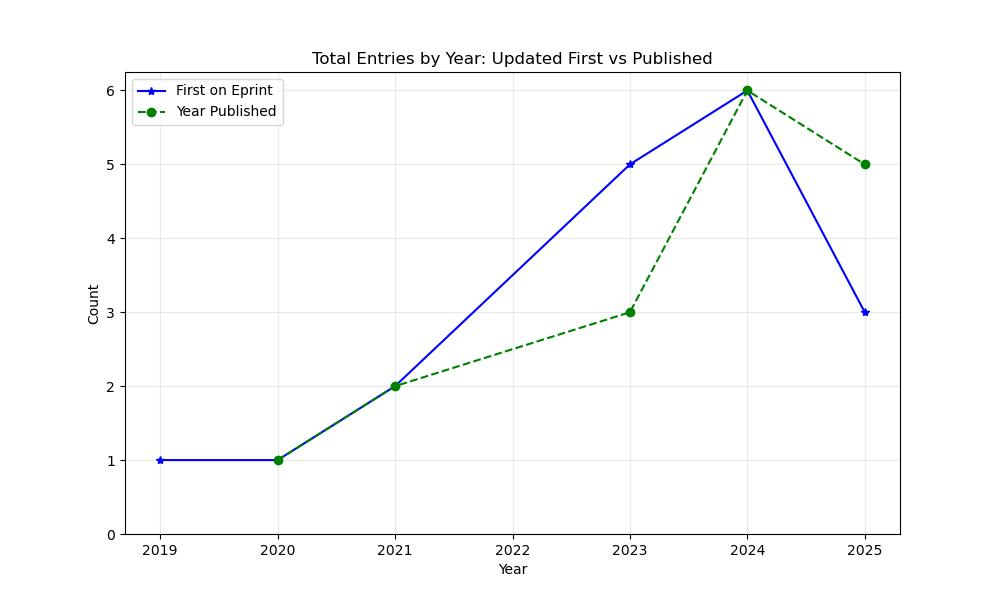
\includegraphics[scale=0.3]{figures/oprf-timeline.jpg}
    \end{column}
  \end{columns}
\end{frame}

\section{MPC recap}

\begin{frame}{A little help from MPC friends}
  \centering
  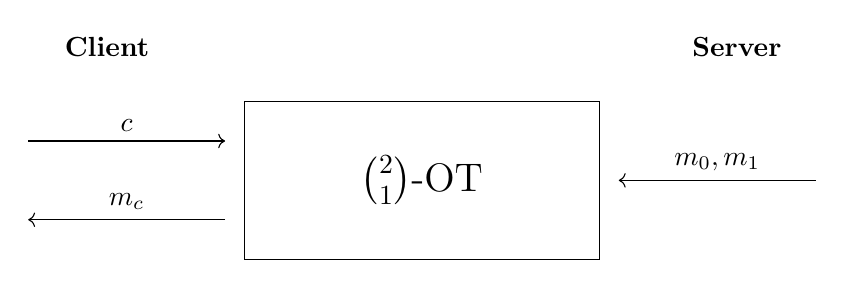
\begin{tikzpicture}
    \node[text centered] at (-4, 1.7) {\textbf{Client}};
    \node[text centered] at (4, 1.7) {\textbf{Server}};

    \node[draw, text centered, minimum width= 4.5cm, minimum height=2cm] at
      (0,0){\Large{$2\choose 1$-OT}};
    \draw[->](5, 0) -- (2.5, 0)node[midway,above]{$m_0, m_1$};

    \draw[->] (-5, 0.5)  -- (-2.5, 0.5) node[midway,above]{$c$};
    \draw[->] (-2.5, -0.5) -- (-5, -0.5) node[midway,above]{$m_{c}$};
  \end{tikzpicture}
  \pause

  \vspace{1em}
  \alert{Extend} with symmetric operations!
\end{frame}

\begin{frame}{A little help from MPC friends (cont.)}
  \centering
  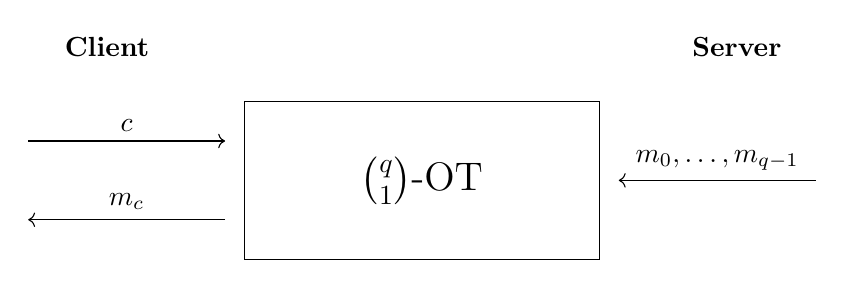
\begin{tikzpicture}
    \node[text centered] at (-4, 1.7) {\textbf{Client}};
    \node[text centered] at (4, 1.7) {\textbf{Server}};

    \node[draw, text centered, minimum width= 4.5cm, minimum height=2cm] at
      (0,0){\Large{$q\choose 1$-OT}};
    \draw[->](5, 0) -- (2.5, 0)node[midway,above]{$m_0, \ldots, m_{q-1}$};

    \draw[->] (-5, 0.5)  -- (-2.5, 0.5) node[midway,above]{$c$};
    \draw[->] (-2.5, -0.5) -- (-5, -0.5) node[midway,above]{$m_{c}$};
  \end{tikzpicture}
\end{frame}

\begin{frame}{A little help from MPC friends (cont.)}
  \centering
  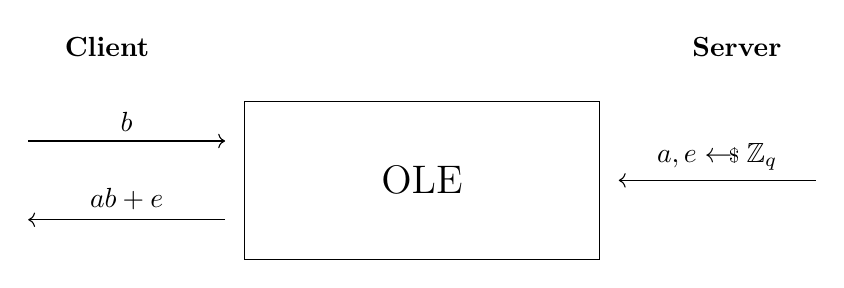
\begin{tikzpicture}
    \node[text centered] at (-4, 1.7) {\textbf{Client}};
    \node[text centered] at (4, 1.7) {\textbf{Server}};
    \node[draw, text centered, minimum width= 4.5cm, minimum height=2cm] at
      (0,0){\Large{OLE}};
    \draw[->](5, 0) -- (2.5, 0)node[midway,above]{$a, e\sample \ZZ_q$};

    \draw[->] (-5, 0.5)  -- (-2.5, 0.5) node[midway,above]{$b$};
    \draw[->] (-2.5, -0.5) -- (-5, -0.5) node[midway,above]{$ab+e$};
  \end{tikzpicture}
  \pause\\
  \emph{Vector variant}\\$\bv{y}=\bv{a}b+\bv{e}$\\ $\bv{a,e,y}\in\ZZ_q^n$
\end{frame}
%%%%%%%%%%%%%%%%%%%%%%%%%%%%%%%%%%%%%%%%%%%%%%%%%%%%%%%%%%%%%%%%%%%%%%%%%%%%%%%
\begin{frame}
  \frametitle{Generics: Evaluating AES, obliviously~\cite{LC:FalOttOtt23}}
  \begin{itemize}
    \item Garble cipher circuit, evaluate with PQ-OT\pause 
    \item $\approx 7 $MB communication\pause
    \item what is missing? \pause
      \begin{itemize}
        \item malicious security\pause
        \item verifiablity\pause
        \item efficient PQ-OT\pause
        \item use MPC-friendly ciphers instead of AES\pause
      \end{itemize}
    \item good baseline! 
  \end{itemize}
\end{frame}
%%%%%%%%%%%%%%%%%%%%%%%%%%%%%%%%%%%%%%%%%%%%%%%%%%%%%%%%%%%%%%%%%%%%%%%%%%%%%%%

%%%%%%%%%%%%%%%%%%%%%%%%%%%%%%%%%%%%%%%%%%%%%%%%%%%%%%%%%%%%%%%%%%%%%%%%%%%%%%%
\sectionheader{Lattice OPRFs}
%%%%%%%%%%%%%%%%%%%%%%%%%%%%%%%%%%%%%%%%%%%%%%%%%%%%%%%%%%%%%%%%%%%%%%%%%%%%%%%
\begin{frame}
  \frametitle{2HashDH, but make it Lattices~\cite{PKC:ADDS21}}
  \begin{figure}[!ht]
    \procedureblock[mode=text]{}{%
      \> \textbf{Client} \> \> \textbf{Server} \((k)\)\\
      \textbf{1. Init:}  \>              \> \sendmessageleft*[22em]{c \coloneqq a \cdot \underline{k} + \underline{e_0},\  a \in \ZZ_{q}[X]/(X^N + 1)} \>\\
      \uncover<2->{
        \textbf{2. Query:} \> Sample short \(\underline{r}\) \> \sendmessageright*[22em]{c_{x}
        \coloneqq H(x) + a \cdot \underline{r} + \underline{e_c}} \> \\
      }
      \uncover<3->{
        \> \(y \coloneqq d_x-c\cdot\underline{r}\) \> \sendmessageleft*[22em]{{d_{x} \coloneqq
            c_{x} \cdot \underline{k} + \underline{e_s} = (H(x) + a \cdot
            \underline{r} + \underline{e_c}
        )\cdot\underline{k} + \underline{e_s}}}
      }
    }
    \uncover<4->{
      \[d_x-c\cdot\underline{r}= H(x)\cdot\underline{k} + a\cdot{rk} +
        \underline{e_c\cdot{k}
      } + \underline{e_s} - a\cdot{rk} - \underline{e_{0} \cdot r} \approx H(x) \cdot {k}\]
    }

    \caption{Generic construction for 2HashDH OPRF from LWE~\cite{PKC:ADDS21}.
    \underline{Underlined} variables are short. }
  \end{figure}
  \hfill\alert{Question} What do we have to prove?
  \vspace{1em}

\end{frame}

%%%%%%%%%%%%%%%%%%%%%%%%%%%%%%%%%%%%%%%%%%%%%%%%%%%%%%%%%%%%%%%%%%%%%%%%%%%%%%%

\begin{frame}{How could a malicious client attack when we forego ZK? }
  \begin{itemize}
    \item Is it safe to output $c_x\bv{k}+\underline{\bv{e}}$ for arbitrary
      $c_x$?\pause ~no, trapdoors!\pause
    \item Noise Leakage: the client learns $\bv{e}_c\bv{k}+\bv{e}_s-\bv{e}_0\bv{ r}$
      where they choose $\bv{e}_0$ and $\bv{r}$ before rounding.\pause
    \item trivial attack:
      \begin{itemize}
        \item Write $\bv{a} \coloneqq (\bv{e}, \bv{-r})$ and $s \coloneqq (\bv{k}, \bv{e}_0)$
        \item Rewrite
          $\bv{e}_c \bv{k} + \bv{e}_0 - \bv{e}_s \bv{r}$
          as $\bv{as} + \bv{e_1}$\pause
        \item This is essentially an instance of \emph{LWE without modular
          reduction}!~\cite{AC:BDEFT18} which is easy. \footnote{
            This is a bit of a simplification because $\bv{e_1}$ is sampled fresh in each
          invocation so the attack does not apply directly.}
      \end{itemize}
  \end{itemize}
\end{frame}

%%%%%%%%%%%%%%%%%%%%%%%%%%%%%%%%%%%%%%%%%%%%%%%%%%%%%%%%%%%%%%%%%%%%%%%%%%%%%%%

\begin{frame}{Client Proof}
  The OPRF requires the client to prove in zero-knowledge that the
  initial message
  $\bv{c}_x \coloneqq H(x) + \bv{ar} + \bv{e}_c$ is \emph{well-formed}.\pause

  More concretely, the client has to prove that:
  \begin{enumerate}
    \item they know an $\bv{x}\in \{0,1\}^\kappa$ \pause
    \item $\bv{r}\in R$ is a small element with $\ll \bv{r} \ll_\infty \leq \sigma \sqrt{n}$\pause
    \item $\bv{e}_c\in R^{1\times \ell}$  where $\ll\bv{e}_c\ll_\infty \leq \sigma
      \sqrt{n}$\pause
  \end{enumerate}
  \alert{Question} Which proof is most expensive? \pause
  The first one. This is the main bottleneck in lattice protocols. 

\end{frame}

% %%%%%%%%%%%%%%%%%%%%%%%%%%%%%%%%%%%%%%%%%%%%%%%%%%%%%%%%%%%%%%%%%%%%%%%%%%%%%%%
% 
% \begin{frame}{Server proof}
%   The server has two proofs:
%   \begin{enumerate}
%     \item in the initialization phase that proves
%       knowledge of a key $\kkk\in R$ and an error term $\bv{e}_0\in R^{1\times
%       \ell}$,\pause ~
%       both of which are shorter elements, \pause and that the key commitment $\bv{c}\coloneqq
%       \bv{a} k +\bv{e}_0$ contains $\bv{a}$
%       such that the commitment is well-formed $\bv{c}=\bv{a}k+\bv{e}_0 \mod q$\pause
%       \begin{itemize}
%         \item can be removed by trapdooring $\kkk$!\pause
%         \item  $\kkk$ has to be extractable, which is also possible by using a
%           trapdoor. However, the proof isn't that bad. \pause
%       \end{itemize}
%     \item  prove that $\bv{d}_x=\bv{c}_x\bv{k}+\bv{e}_s \mod q$ \\
%       can be amortized with batching and generically performed with cut-and-choose
%       (foregoes round-optimality)
% 
%   \end{enumerate}
% \end{frame}
% 
%%%%%%%%%%%%%%%%%%%%%%%%%%%%%%%%%%%%%%%%%%%%%%%%%%%%%%%%%%%%%%%%%%%%%%%%%%%%%%%

\begin{frame}{Modulus requirements for \cite{PKC:ADDS21}}
  \begin{enumerate}
    \item correctness requirements on the ring modulus
      \begin{itemize}
        \item semihonest: 256-bit modulus and a ring dimension of $2^{14}$, which sums to about 2MB
          of communication (over 0.5 MB per ring element). \pause
        \item malicious secure correctness: 2048 bit modulus \pause
          % prevent adversaries from maliciously sampling $k$ such that
          % $H(x)k$ produces a rounding error. 1D-SIS assumption requires $q \gg
          % 2^{2\lambda}$. \pause
      \end{itemize}
    \item Statistical Noise Drowning

      \begin{itemize}
        \item \alert{Question} What is the size of the error terms $\bv{e}_c,
          \bv{e}_s$ ? \pause
        \item have to be small in relation to $q$: \\
          $
          q \overset{\text{correctness of }\approx}{\gg} \bv{e}_s
          \overset{\text{hide } \bv{k}}{\gg} \bv{e}_c \cdot \bv{k}
          $\pause
      \end{itemize}
        \end{enumerate}
\end{frame}

%%%%%%%%%%%%%%%%%%%%%%%%%%%%%%%%%%%%%%%%%%%%%%%%%%%%%%%%%%%%%%%%%%%%%%%%%%%%%%%

\begin{frame}{Reducing server noise~\cite{AC:AlbGur24}}
  \begin{itemize}
    \item avoid 1D-SIS assumption by adding output of random oracle to client
      input
    \item remove superpolynomial dependency on the norm of
      additive terms using Rényi Noise Drownings \pause
    \item Impact on game-based proof: 
      search
      instead of a distinguishing game\pause
    \item bound on number of queries
    \item a few other tricks: Labrador for proofs. \pause
    \item \cite{PKC:ADDS21} $\approx$ 128 GB per evaluation using \cite{C:YAZXYW19}\pause
    \item \cite{AC:AlbGur24}: $\approx$ 538 kB per evaluation using \cite{C:BeuSei23}
  \end{itemize}
\end{frame}

%%%%%%%%%%%%%%%%%%%%%%%%%%%%%%%%%%%%%%%%%%%%%%%%%%%%%%%%%%%%%%%%%%%%%%%%%%%%%%%

\begin{frame}{Further size reductions in Leopard~\cite{EPRINT:ESTX24}}
  \begin{itemize}
    \item 
      Computational Assumption $\ll\bv{e'}\ll \geq poly(\lambda)\sqrt{Q}\ll
      \bv{e}k-\bv{e''}\bv{r}\ll$ \cite{EPRINT:ESTX24}\pause
    \item 
      new assumption iMLWE-RU-R+MLWE+MSIS\pause
  \begin{itemize}
    \item 222 kB~\cite{AC:AlbGur24} to 159 kB online\pause 
    \item 316 kB~\cite{AC:AlbGur24} to 20 kB preprocessing
  \end{itemize}
  \end{itemize}
\end{frame}

%%%%%%%%%%%%%%%%%%%%%%%%%%%%%%%%%%%%%%%%%%%%%%%%%%%%%%%%%%%%%%%%%%%%%%%%%%%%%%%

\begin{frame}
  \frametitle{Pool OPRF~\cite{CCS:DavDeoThi25}}
  \begin{itemize}
    \item \emph{binary} LWR: $\lfloor H(x)^T\cdot k\rceil_p$, $H:
      \{0,1\}^*\mapsto \ZZ_q^n, k\in \{0,1\}^n$\pause
    \item 12 kB, round-optimal, semi-honest\pause
    \item same problem with proving the hash, new assumption
  \end{itemize}
\end{frame}

%%%%%%%%%%%%%%%%%%%%%%%%%%%%%%%%%%%%%%%%%%%%%%%%%%%%%%%%%%%%%%%%%%%%%%%%%%%%%%%

\sectionheader{Naor-Reingold Constructions} % dark background
\begin{frame}{Naor-Reingold PRF~\cite{NaoRei04}}
  \begin{itemize}
    \item The Naor-Reingold PRF~\cite{NaoRei04} that generically builds a PRF
      from an Abelian group action $*$.
      \item
      To compute the PRF over $m$ input bits, we sample $m+1$ group elements $[g_0,
      g_1, \ldots, g_m]$. \pause
    \item Start with group action with $g_0$\pause
    \item For every following
      group element, the group action is performed when the $i^{th}$ bit of the input is set. \pause
  \end{itemize}
  \begin{example}[Naor-Reingold with seven input bits]
    For example, for $0110111$ we would
    compute the group action $g_0*g_2*g_3*g_5*g_6*g_7$.
  \end{example}
\end{frame}

%%%%%%%%%%%%%%%%%%%%%%%%%%%%%%%%%%%%%%%%%%%%%%%%%%%%%%%%%%%%%%%%%%%%%%%%%%%%%%%

\begin{frame}{PRF from rounded Subset-Product over Rings}
  \begin{itemize}
    \item 2014: SPRING~\cite{FSE:BBLPR14}, an LWR-style PRF with small modulus\pause
    \item focus in \textsc{Spring-BCH}: $q=257$, rounding bias reduction using extended BCH code
      $[128,64,22]$\pause
    \item Oblivious evaluation: 304 bytes/ 11$\mu$s client, 22 kB/227 $\mu$s server
  \end{itemize}

  \onslide<3-6>{
    \begin{figure}[H]
      \label{Spring:PRF}
      \vspace{-1em}
      \begin{align*}
        \mathcal{F}_{\bv{K}}(c_1,
        \cdots,c_m)=S\left(\kkk_0 \prod_{i=1}^m \kkk_{i}^{c_i}\right)
      \end{align*}
    \end{figure}
  }

  \onslide<7>{
    \begin{figure}[H]
      \label{Spring:PRF-intt}
      \vspace{-8em}
      \begin{align*}
        \mathcal{F}_{\bv{K}}(c_1,
        \cdots,c_m)=S\left(\iNTT\left(\kkk_0\cdot \prod_{i=1}^m \kkk_{i}^{c_i}\right)\right)
      \end{align*}
    \end{figure}
  }

  \onslide<8>{
    \begin{figure}[H]
      \label{Spring:PRF-intt-lookup}
      \vspace{-8em}
      \begin{align*}
        \mathcal{F}_{\bv{K}}(c_1,
        \cdots,c_m)=S\left(\iNTT\left(\mathsf{lookup}\left(\kkk_0+
        \sum_{i=1}^m {c_i}\kkk_{i}\right)\right) \right)
      \end{align*}
    \end{figure}
  }

\end{frame}

\begin{frame}
  \frametitle{lattice-ish OPRF overview}
  \begin{tabular}{cccccc}
    Construction & rounds & malicious secure & comms & preprocessing 
    \\\hline
    \cite{PKC:ADDS21} & 2 & \faTimes & 2MB & /  \\
    \cite{PKC:ADDS21} & 2 & \faCheck & 128 kB & /  \\
    \cite{AC:AlbGur24} & 2 & \faCheck & 	222 kB & 	316 kB ($2^{6}$ queries) \\
    \cite{EPRINT:ESTX24} & 2 & \faCheck & 159 kB &20 kB \\
    \cite{CCS:DavDeoThi25} & 2 & \faTimes & 	12 kB & 1.5 MB (amortizable) \\
    \cite{EC:HKLMRR25} & 6& \faTimes &  23 kB &  793 kB (amortizable) \\
  \end{tabular}
\end{frame}
 
%%%%%%%%%%%%%%%%%%%%%%%%%%%%%%%%%%%%%%%%%%%%%%%%%%%%%%%%%%%%%%%%%%%%%%%%%%%%%%%

\sectionheader{Isogenies}

%%%%%%%%%%%%%%%%%%%%%%%%%%%%%%%%%%%%%%%%%%%%%%%%%%%%%%%%%%%%%%%%%%%%%%%%%%%%%%%
\begin{frame}\frametitle{2HashDH from SIDH~\cite{SAC:Basso23}}
  \begin{columns}[c]
    \begin{column}{.49\textwidth}
  \begin{itemize}
    \item repairs 2HashDH construction~\cite{AC:BonKogWoo20} from SIDH isogenies\pause
    \item No MPC!\pause
    \item malicious security \pause
    \item round-optimal\pause
    \item 
      8.7 MB comms
  \end{itemize}
    \end{column}
    \begin{column}{.49\textwidth}
      \uncover{1-}{
      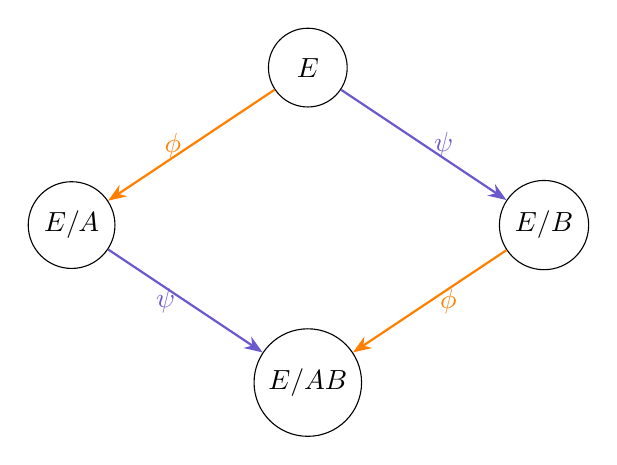
\begin{tikzpicture}[
    node distance=3cm,
    curve/.style={circle, draw, minimum size=1cm},
    arr/.style={-Stealth, thick},
]

% Curves
\node[curve] (E0) at (0,0) {$E$};
\node[curve] (EA) at (-3,-2) {$E/A$};
\node[curve] (EB) at (3,-2) {$E/B$};
\node[curve] (EAB) at (0,-4) {$E/{AB}$};

% Alice's path
\draw[arr, orange] (E0) -- node[left] {$\phi$} (EA);
\draw[arr, thirdColor] (EA) -- node[left] {$\psi$} (EAB);

% Bob's path
\draw[arr, thirdColor] (E0) -- node[right] {$\psi$} (EB);
\draw[arr, orange] (EB) -- node[right] {$\phi$} (EAB);


\end{tikzpicture}
}
    \end{column}
    \end{columns}
\end{frame}

%%%%%%%%%%%%%%%%%%%%%%%%%%%%%%%%%%%%%%%%%%%%%%%%%%%%%%%%%%%%%%%%%%%%%%%%%%%%%%%


 \begin{frame}[t]{CSIDH in one slide}
   \begin{minipage}{.5\textwidth}
     \begin{itemize}
       \item random walk on commutative graph
       \item node: curve with Montgomery coefficient
       \item private key describes number of steps and orientation
     \end{itemize}
   \end{minipage}
   \begin{minipage}{.35\textwidth}
     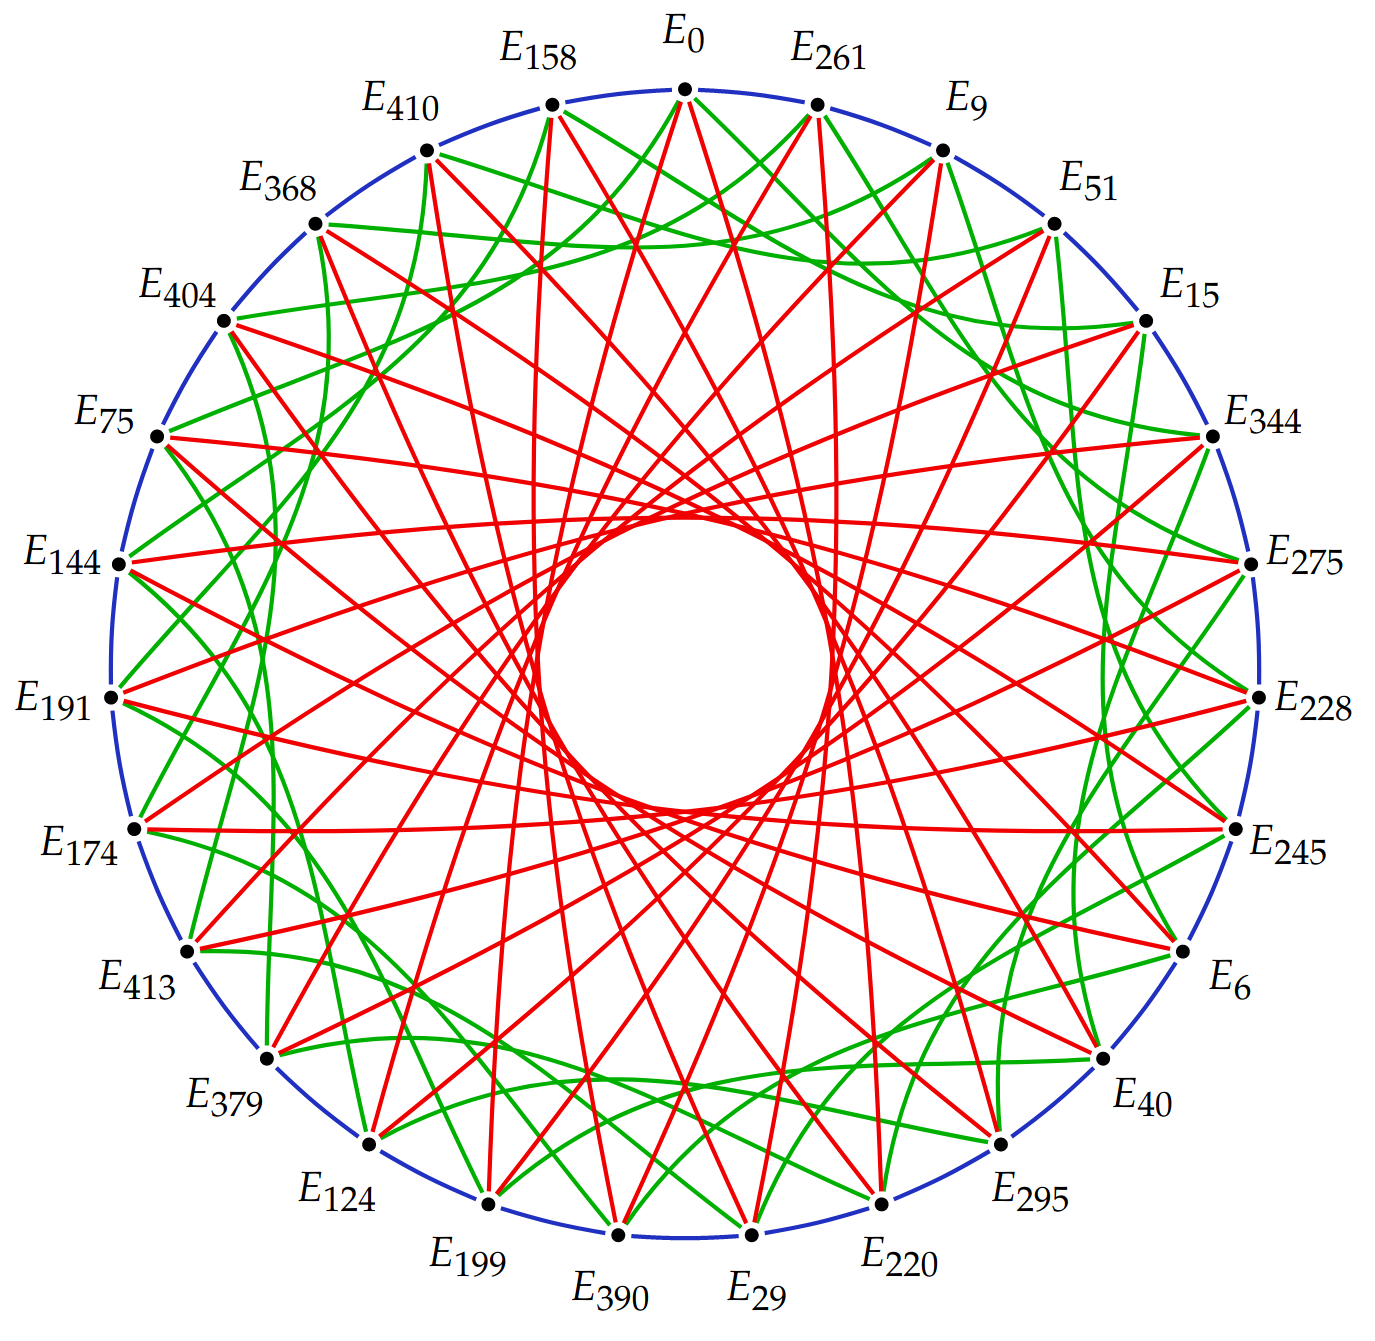
\includegraphics[scale=0.2]{figures/isogenies.png}
   \end{minipage}
 \end{frame}


\begin{frame}\frametitle{Naor-Reingold OPRF from CSIDH}
  \begin{itemize}
    \item blind key and reduce via \emph{relational
      lattice}~\cite{ASIACCS:HHMRR24,PKC:DelPed24}\pause
    \item CSIDH OT needs trusted setup \pause \\ $\rightarrow$ doesn't exist for
      CSIDH\pause
    \item Explicit consecutive evaluation: OPUS~\cite{ASIACCS:HHMRR24}, no
      trusted setup, no class group structure\pause
  \end{itemize}

  \centering
  \begin{tabular}
  {llllll}
  \toprule
  protocol &  rounds & comm. cost& isog. comp. & model (C-S)\\
  \midrule
  NR-OT& $2$ & $2\sigma \cdot \gamma +2\gamma^2+\sigma$& $5\gamma+2$
       &\halfcirc-\halfcirc\\
  NR-OT& $4$ & $5\sigma\cdot\gamma + 5\gamma^2+\sigma$&  $11\gamma+2$  &
  \fullcirc-\halfcirc
  \\
  OPUS&$2\gamma+2$& $3\sigma\cdot\gamma+2\sigma$ &$3\gamma+3$&
  \halfcirc-\halfcirc \\
  \cite{PKC:DelPed24} & 2 & $(\lambda+5)\gamma+2\lambda$  &$4\lambda +2$ & \fullcirc-\halfcirc\\ 
  \bottomrule
\end{tabular}

  \vspace{1em}

  $\gamma$ input bits, $\rho$ CSIDH modulus
\end{frame}

%%%%%%%%%%%%%%%%%%%%%%%%%%%%%%%%%%%%%%%%%%%%%%%%%%%%%%%%%%%%%%%%%%%%%%%%%%%%
%%%%%%%%%%%%%%%%%%%%%%%%%%%%%%%%%%%%%%%%%%%%%%%%%%%%%%%%%%%%%%%%%%%%%%%%%%%%%%%
\sectionheader{Legendre OPRFs}
%%%%%%%%%%%%%%%%%%%%%%%%%%%%%%%%%%%%%%%%%%%%%%%%%%%%%%%%%%%%%%%%%%%%%%%%%%%%%%%
%%%%%%%%%%%%%%%%%%%%%%%%%%%%%%%%%%%%%%%%%%%%%%%%%%%%%%%%%%%%%%%%%%%%%%%%%%%%%%%

\begin{frame}
  \begin{definition}[Legendre Symbol]
    An integer $a$ is a quadratic residue mod $p$ if the equation $x^2\equiv a
    \mod p$ is solvable and $\text{gcd}(a,p)=1$.
    The Legendre symbol for some integer $a$ and an odd prime $p$ is
    \begin{align*}
      \left(\frac{a}{p}\right)=\begin{cases} 
        1 & \text{if } a \text{ is a quadratic residue mod } p\\
        -1 & \text{if } a \text{ is a quadratic non-residue mod } p\\
        0 & \text{if } a \equiv 0 \mod p
      \end{cases}
    \end{align*}
  \end{definition}
\end{frame}

%%%%%%%%%%%%%%%%%%%%%%%%%%%%%%%%%%%%%%%%%%%%%%%%%%%%%%%%%%%%%%%%%%%%%%%%%%%%%%%

\begin{frame}
  \frametitle{Legendre PRF}
  \begin{definition}[Legendre PRF~\cite{C:Damgard88a}]
    \begin{align*}
    F_k(x)\coloneqq (k+x)^{\frac{p-1}{2}}
    \end{align*}
  \end{definition}\pause
    $x=-k$: $F_k(x)=0$, distinguisher in OPRF setting\pause
   \begin{definition}[Sequential Legendre PRF]
     \begin{align*}
      % L_K(x)\coloneqq \lfloor \frac{1}{2}\left( 1-\frac{K+x){p}\right)\lfloor
       \{a\}_K\coloneqq
       \left(\frac{K}{p}\right),\left(\frac{K+1}{p}\right),\ldots,\left(\frac{K+a-1}{p}\right)
     \end{align*}
   \end{definition}
\end{frame}

%%%%%%%%%%%%%%%%%%%%%%%%%%%%%%%%%%%%%%%%%%%%%%%%%%%%%%%%%%%%%%%%%%%%%%%%%%%%%%%

\begin{frame}
  \frametitle{A straightforward Legendre OPRF~\cite{SerHorBur23}}
  \begin{itemize}
    \item oblivious evaluation using a trusted third party for 
  \begin{itemize}
    \item Beaver triples to multiply additively shared values
    \item perfect square $s^2$ for shared Legendre symbol computation
  \end{itemize}
    \item $\approx 13$kB online, expensive preprocessing
  \end{itemize}
\end{frame}

%%%%%%%%%%%%%%%%%%%%%%%%%%%%%%%%%%%%%%%%%%%%%%%%%%%%%%%%%%%%%%%%%%%%%%%%%%%%%%%

\begin{frame}
  \frametitle{Explicit distributed construction~\cite{ESORICS:KalCheMit25}}
  \begin{itemize}
    \item replicated secret sharing for fast online multiplications (semihonest
      variant)\pause
    \item avoids zero-knowledge proofs, but requires checks in precomputation\pause
    \item doubly replicated secret sharing for malicious security: not
      round-optimal \pause
    \item concrete performance depends on number of corrupted servers
   %  \item 2 varianten, jeweils 1x SH 1x malicious, nur die mit dem replicated
   %    secret sharing ist implementiert. es gibt optimized secret sharing, ist
   %    nicht round-optimal (1x comms zwischen client und server)
   %  \item replicated secret sharing: additive secret sharing, jeder server hat
   %    an share. 
   %    replicated: jeder server hat mehrere shares, viel über indices. jeder
   %    server kriegt jeden share wo kein eigener share drinnen is. 
  \end{itemize}
\end{frame}

%%%%%%%%%%%%%%%%%%%%%%%%%%%%%%%%%%%%%%%%%%%%%%%%%%%%%%%%%%%%%%%%%%%%%%%%%%%%%%%
 \begin{frame}
   \frametitle{Frame, then build: 2HashDH UC Framework \cite{EC:BDFH25}}
   \begin{itemize}
     \item sequential Legendre PRF well-proven in UC \pause
     \item general idea: use perfect square $a^2$ to mask  
       $K+h+l_i'$ since $\left(\frac{a\cdot b}{p}\right)=\left(\frac{a}{p}\right) \left(\frac{b}{p}\right)$\pause
        \begin{itemize}
          \item server samples random vector $\bv{a}$ and defines
            \begin{align*}\bv{u}=\{(K+l_i')a_i^2\}_{i\in [\ell_{eval}]}\text{ and }
              \bv{v}=\{a_i^2\}_{i\in [\ell_{eval}]}\end{align*}\pause
              \item VOLE computes $$\bv{o}\coloneqq
                \bv{u}+h*\bv{v}=\{(K+h+l_i')a_i^2\}_{i\in [\ell_{eval}]}$$\pause
              \item user receives $o_i=(K+h+l_i')a^2$ and can compute $$
                \left(\frac{o_i}{p}\right)=
                \left(\frac{(K+h+l_i')a_i^2}{p}\right)=
                \left(\frac{K+h+l_i'}{p}\right)
                $$
        \end{itemize}
   \end{itemize}
 \end{frame}

%%%%%%%%%%%%%%%%%%%%%%%%%%%%%%%%%%%%%%%%%%%%%%%%%%%%%%%%%%%%%%%%%%%%%%%%%%%%%%%

\begin{frame}
  \frametitle{Gold OPRF~\cite{SP:YBHKR25}}
  \begin{itemize}
    \item Power Residue PRF: Generalization of Legendre PRF $(k+x)^g\mod p$, $p=2^\lambda
      \cdot g +1\in \mathbb{P}$ to get $\approx \mathcal{O}(\lambda)$
      output instead of a single bit. \pause
    \item for PQ security, $p$ needs to be $>384$ bits\pause
    \item VOLE correlations to compute PRF obliviously\pause
    \item three variants: 
      \begin{itemize}
        \item 2PC-Gold (reverse DLOG): $(k+x)^g$, $k,x$ are private\pause
        \item O-Gold: more 2HashDH-style $H_2(x,\text{Gold}_k(H_1(x)))$\pause\\
          performance similar to 2PC-Gold
        \item UC gold: UC provable, removes edge case of $x=-k$
      \end{itemize}
    \item three rounds of communication
  \end{itemize}
\end{frame}


\begin{frame}
  \frametitle{Legendre OPRF overview}
  \begin{tabular}{ccccc}
    Construction & rounds & malicious secure & comms & preprocessing 
    \\\hline
    \cite{ESORICS:KalCheMit25} & 2 & \faTimes & 144 kB & 432 kB  \\
    \cite{EC:BDFH25} & 9 & \faCheck & 	356 kB & 	392 kB \\
    \cite{SP:YBHKR25} & 3& \faCheck &  970 kB (1.9 kB) & -  \\
  \end{tabular}
\end{frame}


%%%%%%%%%%%%%%%%%%%%%%%%%%%%%%%%%%%%%%%%%%%%%%%%%%%%%%%%%%%%%%%%%%%%%%%%%%%%
%%%%%%%%%%%%%%%%%%%%%%%%%%%%%%%%%%%%%%%%%%%%%%%%%%%%%%%%%%%%%%%%%%%%%%%%%%%%%%%
\sectionheader{Alternating Moduli constructions}
%%%%%%%%%%%%%%%%%%%%%%%%%%%%%%%%%%%%%%%%%%%%%%%%%%%%%%%%%%%%%%%%%%%%%%%%%%%%%%%
%%%%%%%%%%%%%%%%%%%%%%%%%%%%%%%%%%%%%%%%%%%%%%%%%%%%%%%%%%%%%%%%%%%%%%%%%%%%%%%

\begin{frame}
  \frametitle{Alternating Moduli PRF}
  \begin{itemize}
    \item linear functions over different moduli (2 and 3)   \pause
    % \item $(n,m,t)$, $m\leq n, t$
    \item $\bv{B}\in\ZZ_3^{t\times m}$ is public, $\bv{K}\in\ZZ_2^{m\times n}$
      is secret, 
    $\bv{x}\in \ZZ_2^n$ is the input, $\bv{y}\in \ZZ_3^n$ is the output\pause
  \item Core idea: use linear maps as high degree functions (i.e. 
        map over $\ZZ_2$ is  a high degree function over $\ZZ_3$ and vice
        versa)\pause
  \begin{enumerate}
    \item compute non-compressive (secret) linear map $\bv{w}=\bv{K}\times
      \bv{x}$\pause
      \item reinterpreted over
      $\ZZ_3$\pause
      \item compute compressive public linear map over $\ZZ_3$ by computing
      $\bv{B}\times\bv{w}=\bv{y}$\pause
  \end{enumerate}
    \item weak PRF: only uniformly random inputs are allowed
  \end{itemize}
\end{frame}

\begin{frame}
  \frametitle{\cite{C:DGHIKS21}}
  \begin{itemize}
    \item new alternating-moduli PRFs, friendly for OT correlations\pause
    \item semi-honest, round-optimal construction\pause \\
     limited usage recommended ($\approx 2^{40}$ evaluations)\pause
    \item (V)OLE for oblivious evaluation\pause
    \item preprocessing for conversion between rings $\mod 2$ to $\mod 3$
    \item subset-sum symmetric hardness\pause
    \item performs better in preprocessing/communication/computation because
      of efficient modulus conversion gates instead of generic OT
  \end{itemize}
\end{frame}

\begin{frame}
  \frametitle{\cite{EC:ADDG24}}
  \begin{itemize}
    \item use torus FHE for malicious security \\ \pause wPRF is MPC and FHE
      friendly!
    \item no preprocessing\pause
    \item not verifiable~\cite{AC:CheoJan25}
  \end{itemize}

\end{frame}

\begin{frame}
  \frametitle{\cite{C:APRR24}}
  \begin{itemize}
    \item \emph{point-wise alternating moduli} PRFs\pause
    \item small signatures, 3/4 constructions broken~\cite{AC:SidWan25}\pause
    \item reverse many-to-one construction: \pause\\ 
      setup + $\approx 130$ bytes comms
  \end{itemize}
\end{frame}
\begin{frame}
  \frametitle{alternating moduli OPRF overview}

  \begin{tabular}{ccccc}
    Construction & rounds & malicious secure & comms & preprocessing 
    \\\hline
    \cite{C:DGHIKS21} & 2 & \faTimes & 80 bytes & 200 bytes  \\
    \cite{EC:ADDG24} & 2 & \faCheck & 	160 kB & 2.5 MB \\
    \cite{C:APRR24} & 2& \faTimes  &  $\approx 130$ bytes & 5
    bytes(amort.)  \\
  \end{tabular}
\end{frame}

\begin{frame}
  \frametitle{Conclusion}
  \begin{itemize}
    \item OPRFs vs. blind signatures? \pause
    \item Find better algebra? \pause
    \item design oblivious-evaluation friendly PRFs\pause 
    \item better MPC techniques + MPC-friendly symmetric primitives (e.g. random
      OT from lattices)\pause
    \item lift semi-honest constructions to malicious
      constructions\pause
    \item We still don't have a great, general-purpose construction! \pause But
      we have good amortizable PRFs.
  \end{itemize}
\end{frame}
\appendix

\begin{frame}{Acknowledgement}
    \begin{exampleblock}{Acknowledgements}
    This presentation was prepared using funds from the Digital Europe Program under grant
  agreement number 101091642 (QCI-CAT).  \end{exampleblock}


\end{frame}

\begin{frame}[allowframebreaks]{References}
  \bibliography{export/abbrev3,export/crypto,bilbio}
  \bibliographystyle{alpha}
\end{frame}

\begin{frame}
  \frametitle{State of blind signatures}
  \begin{figure}
    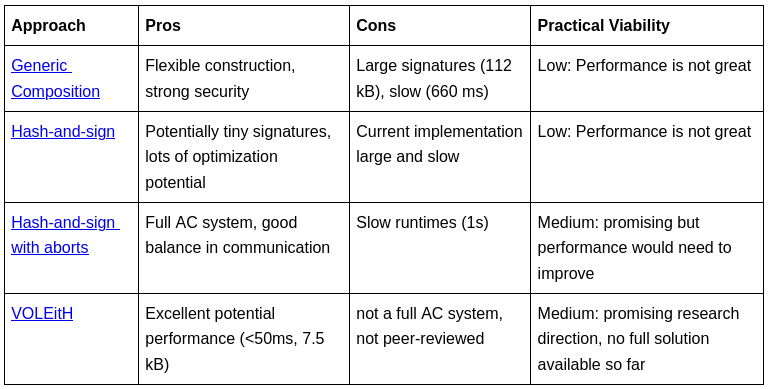
\includegraphics[scale=0.5]{figures/blind-signatures.png}
    \caption{Blind signatures in the context of anonymous credentials~\url{https://blog.cloudflare.com/pq-anonymous-credentials/}}
  \end{figure}
\end{frame}

\end{document}
